
%%%%%%%%%%%%%%%%%%%%%%%%%%%%%%%%%%%%%%%%%%%%%%%%%%%%%%%%%%%%%%%%%%%%
%%%%%%%%%%%%%%%%%%%%%%%%%%%%%%%%%%%%%%%%%%%%%%%%%%%%%%%%%%%%%%%%%%%%
\chapter{GENFORM} \label{genform}



% ==================================================================
\section{What is GENFORM?}

GENFORM means “generic form” and is a WebObs integrated tool to create a \wo{form} with user-defined database fields, configurable form layout and display/export table of selected data. The form can be associated to a \wo{proc} which define the associated \wo{nodes}. Each record is associated to a single \wo{node} of the \wo{proc}. Data associated to a GENFORM can be read by the proc without the need of defining RAWFORMAT and RAWDATA.

When creating a new \wo{form}, you can define it from a selection of various templates, and modify it as you wish. Once created, a \wo{form} can be modified by adding new inputs and/or change the form layout, but previous inputs cannot be deleted: if an input is not used anymore, it can be ignored and remove from the form layout fields.

A GENFORM is defined by its configuration file (based on the \wokey{key|value} model) with a specific syntax defining the input fields (name, unit and type) and form layout. Each \wo{form} is then associated to a table in a database called \wofile{WEBOBSFORMS.db}. Each table of the database use the scheme shown in table \ref{table:genform_db}.

\begin{table}
	\centering
	\begin{tabular}{c c l}
		\hline
		\textit{Name} & \textit{Type} & \textit{Comment} \\
		\hline
		{\tt id}         & integer  & primary key autoincrement\\
		{\tt trash}      & boolean  & True = bin	\\
		{\tt node}       & text     & WebObs ID of the associated \wo{node} \\
		{\tt edate}      & datetime & date and time end of measurement/collect/sampling \\
		{\tt edate\_min} & datetime & uncertainty date and time end of measurement \\
		{\tt sdate}      & datetime & date and time of optional start of measurement \\
		{\tt sdate\_min} & datetime & uncertainty date and time start of measurement \\
		{\tt users}      & text     & WebObs UID or GID of the operators (authorized list) \\
		{\tt input01}    & text     & data n°1 \\
		{\tt input02}    & text     & data n°2 \\
		...              & text     & data n°... \\
		{\tt comment}    & text     & \\
		{\tt tsupd}      & timestamp & last edit timestamp \\
		{\tt userupd}    & text     & last edit user UID \\
		\hline
	\end{tabular}
	\caption{Scheme of the GENFORM database (each table).}
	\label{table:genform_db}
\end{table}


\section{Creation of a FORM} \label{genform_creation}

To create a new \wo{form} using GENFORM, you have to go in the \wo{grid} menu list and click on the pencil next to \textbf{Raw Data}. Then, you have to choose a name for the FORM and select a template that will be used to help you through the creation process. Currently, 3 templates exist:

\begin{itemize}
	\item GENFORM: the most basic template that shows you all the different types of inputs that you can use in GENFORM
	\item WATERS: a template based on the former EAUX \wo{form} used for the water chemistry analysis
	\item VOLCGAS: a template based on the former GAZ \wo{form} used for the gas chemistry analysis
\end{itemize}

\begin{figure}[!h]
	\centering
	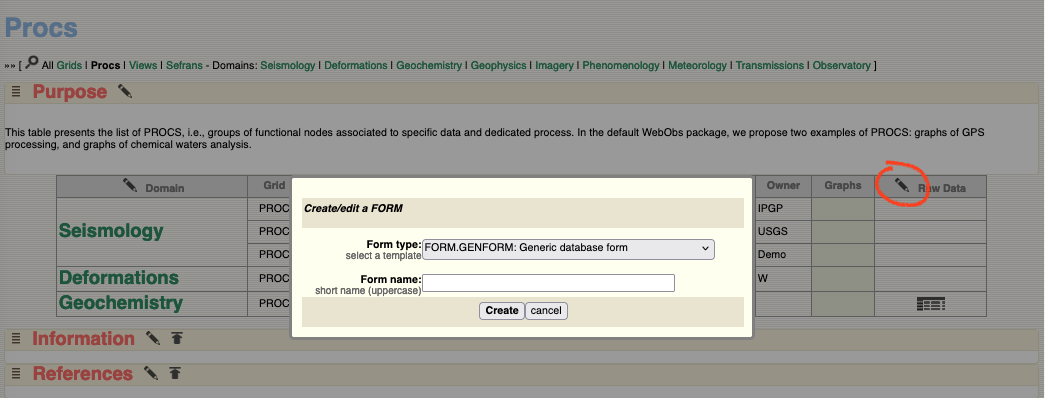
\includegraphics[width=\textwidth]{figures/GENFORM_creation.png}
	\caption{To create a form, click on the edit pencil, choose a template in the list and enter a short name.}
	\label{GENFORM_creation}
\end{figure}

If you want to edit a \wo{form}, you just need to go in the GENFORM creation menu and write the name of the \wo{form} you want to edit, no matter the template which is selected (see figure \ref{GENFORM_creation}).

\section{The GENFORM language}

The GENFORM form layout is separated into \wokey{COLUMNS} number of columns, and a total of \wokey{FIELDSETS} field sets. Each field xx set contains \wokey{FIELDSET\_xx\_COLUMNS} sub-columns, and each sub-column contains several fields of inputs \wokey{INPUTxx} or outputs \wokey{OUTPUTxx}. Inputs and outputs fields have a NAME (mandatory), and optional UNIT, TYPE, THRESHOLD, and HELP.

The NAME contains the full name of the field, but it is recommended to use short names since it will be used in the table column header.

The UNIT contains unit of the field (if revelant).

Valid types for an INPUT field are:
\begin{itemize}
	\item \wokey{text(size)} : text string, optional size in characters (default is 5);
	\item \wokey{numeric(size)}: numeric input, optional size in characters (default is 5);
	\item \wokey{list:\textit{filename}}: points to a config file containing a \wokey{key|value} list of selectable items.
\end{itemize}

Valid types for an OUTPUT field are:
\begin{itemize}
	\item \wokey{formula(size):\textit{formula}}, which allows to make simple mathematical operations between the different inputs and/or outputs. Optional size of the result in characters (default is 6), and size$-3$ significant digits;
	\item \wokey{text} : text string (HTML allowed).
\end{itemize}

The THRESHOLD applies to input or output of numeric/formula types. It contains a coma-separated list of 2 threshold values {\it a, b} to display color background associated to a level of validity of the field absolute value. Three levels are defined: normal (green), warning (orange), and error (red). The criteria are, where {\it x} is the field value:
\begin{itemize}
	\item normal for abs({\it x}) $<=$ {\it a},
	\item warning for {\it a} $<$ abs({\it x}) $<=$ {\it b},
	\item error for abs({\it x}) $>$ {\it b}.
\end{itemize}

The 3 threshold colors can be defined in \wokey{THRESHOLD\_COLORS} variable, for normal, warning, and error levels, respectively. Note that normal level color applies only in the form; for table display of data the normal level value has no background color (for readability).

Each FIELDSET has a NAME, a number of CELLS dividing it, and the NAME of the fields (INPUT or OUTPUT) you want to display in each CELL. CELLS are arranged into columns (the default), or into rows inside the FIELDSET. Finally, each CELL has a list of the fields you want to display in: fields are arranged vertically in the CELL if the FIELDSET is splitted into columns, or horizontally if splitted into rows.

Finally, the configuration file of the \wo{form} has:
\begin{itemize}
	\item a \wokey{TITLE} (long string),
	\item a \wokey{BANG}, which is the oldest year of potential record in the \wo{form},
	\item a \wokey{STARTING\_DATE} flag which is a boolean, allowing GENFORM to define a starting date of each record in addition to end date,
	\item an \wokey{OPERATORS\_LIST}, list of operators as user UIDs and/or group +GIDs.
\end{itemize}

% ==================================================================

\begin{table}[htp]
\caption{GENFORM template}
\label{genform_template}
\lstinputlisting{../../CODE/tplates/FORM.GENFORM}
\end{table}


